
%%% Capítulo 2 - Aspectos Matemáticos

\chapter{Aspectos Matemáticos dos\\Modelos de Complexidade Social}
\label{ch:C2}
% \chapquote{
% }{}

Este capítulo se compromete com a introdução dos conceitos matemáticos básicos na elaboração de modelos para explicar o comportamento social.
Espera-se, contudo, que o leitor esteja familiarizado com a linguagem do cálculo diferencial e integral em várias variáveis e tenha boa noção dos conceitos de probabilidade e estatística.
Dito isso, o tratamento dos tópicos neste capítulo está longe de ser considerado completo ou rigoroso, tendo como principal função uma de referência para a interpretação e análise dos resultados
apresentados no capítulo \ref{ch:C3}.
Um tratamento mais abrangente do estudo de aprendizado de máquinas pode ser encontrado em \parencite{Engel2001}, enquanto tópicos específicos de teoria de grafos podem ser estudados em \parencite{NewmanBook}.

Começaremos com uma breve revisão da teoria de \emph{Aprendizado de Máquina}, introduzimos as linguagens da \emph{Teoria de Grafos} e da \emph{Mecânica Estatística}.
Em seguida, elaboramos o conceito de \emph{Modelos de Agentes}
e estabelecemos o contexto de sua aplicação em sistemas sociais através da identificação das características observadas na realidade com os elementos do modelo.
Finalmente, uma análise de campo médio é feita para obter uma previsão teórica do que se espera do modelo.

\section{Aprendizado de Máquina}
\label{sec:ML}

A investigação de fenômenos sociais demanda uma certa compreensão de \emph{indivíduo} e suas relações com seu arredores e com os demais indivíduos.
Uma pessoa é, por si, um sistema altamente complexo, e a riqueza do comportamento humano torna impraticável a elaboração de uma representação matemática perfeita para o indivíduo.
Todavia, é possível focar nas caraterísticas que pareçam, em uma primeira aproximação, mais relevantes para a compreensão do fenômeno em estudo.
Por exemplo, para compreender o comportamento de multidões em trânsito, a posição e a estratégia para se mover são mais relevantes do sua opinião sobre política, entretanto esta se torna mais importante num contexto de eleições.
Para abordar fenômenos sociais relacionados à diversidade de opiniões ou ideologias políticas, parece razoável dar foco no modo cada indivíduo constrói e representa esses conceitos.

\subsection{Aprendizado Supervisionado \emph{Online}}
\label{ssec:SOL}
Como visto no capítulo \ref{ch:C1}, comportamento social é aprendido e a imitação de comportamento é uma das formas pela qual aprendizado se dá\footnote{veja o capítulo \ref{ch:C1} para mais detalhes.}.
O estudo do Aprendizado de Máquina, em particular o de \emph{aprendizado supervisionado}, será adequado para a descrever o comportamento de indivíduos em contato num contexto de troca de \emph{opiniões}.

\newcommand{\Dt}{\ensuremath{D_t}} \newcommand{\rl}{\ensuremath{\vec{w}}}
\newcommand{\wt}{\ensuremath{\estv{w}}} \newcommand{\wT}{\ensuremath{\wt_+}}
A construção dessa associação é feita estabelecendo o cenário de aprendizado \emph{aluno-professor}.
Tanto professor quanto aluno são representados por vetores $K$-dimensionais, $\rl,\wt \in R^K$, envolvidos na discussão de questões $\vec{x}_a \in \R^K$, também representadas por vetores no mesmo espaço.
Cada exemplo do conjunto $\Dt = \{y_i,\dots,y_t\}$ é composto por uma \emph{`questão`} $\vec{x}_a$ e uma resposta $\tau_a$ a ela dada pelo professor.
Os exemplos em $D_t$ são independentes entre si e identicamente distribuídos pela $P(y_a|\rl)=P(\tau_a|\vec{x}_a\,\rl)P(\vec{x}_a)$.
Através do conjunto de exemplos $D_t$, o aluno $\wt$ tentará aprender o comportamento do professor $\rl$.

Usando o teorema de \emph{Bayes} temos \begin{equation}\label{eq:bayes}
  P(\rl|\Dt) = \frac{Q(\rl)P(\Dt|\rl)}
                    {\int \msr{\rl'} Q(\rl')P(\Dt|\rl')}
\end{equation}
onde $Q(\rl)$ é uma distribuição à priori para \rl.
Considere a apresentação de um novo exemplo $y_{t+1}=y=(\tau,\vec{x})$ ao conjunto $\Dt$, independente dos demais.
A postura no aprendizado Bayesiano é assumir a distribuição à posteriori $P(\rl|\Dt)$ obtida com os exemplos anteriores como a priori $Q(\rl|\Dt)$ sobre a apresentação do novo exemplo.
Com isso, a atualização da distribuição fica
\begin{align}\label{eq:bayes-update}
  P(\rl|y\,\Dt) & = \frac{Q(\rl|\Dt)P(y|\rl)}
       {\int \msr{\rl'} Q(\rl'|\Dt)P(y'|\rl')} \notag \\
  & = \frac{Q(\rl|\Dt)P(\tau|\vec{x}\,\rl)}
           {\int \msr{\rl'} Q(\rl'|\Dt)P(\tau|\vec{x}\,\rl')}
\end{align}
onde foi usado o fato do novo exemplo também ser independente dos demais, ou seja,
\[
P(y,\Dt|\rl) =
P(y|\Dt\,\rl)P(\Dt|\rl) =
P(y|\rl)P(\Dt|\rl)
\]
e o fato de $P(x)$ ser independente de $\rl$.

\newcommand{\Ct}{\ensuremath{\vec{C}}}
\newcommand{\CT}{\ensuremath{\Ct_+}}
\newcommand{\At}{\ensuremath{\theta}}
\newcommand{\AT}{\ensuremath{\At_+}}
O custo computacional de armazenar o conjunto de exemplos e computar a atualização da distribuição posterior crescem a cada apresentação de um novo exemplo.
Seria interessante, do ponto de vista da eficiência computacional \footnote[][-4cm]{Não apenas do ponto de vista tecnológico, mas também como uma   questão evolutiva.
Imagine que os indivíduos de uma espécie tenham evoluído   sua capacidade de armazenar memória e inferir sobre fontes de perigo com base nas suas experiências de vida.
Ambas tarefas tem um custo energético, demandam tamanho cerebral e têm influência direta na sobrevivência dos indivíduos, então é de se esperar que espécies mais eficientes tenham vantagem, num contexto de seleção natural, quando em competição com outras menos eficientes.
Para uma abordagem interessante da evolução de programas veja \parencite{Neirotti2003,Neirotti2006}}, ser capaz de fazer boa inferência com base nos exemplos sem a inconveniência advinda do tamanho do seu conjunto.
Para isso, faremos uma aproximação gaussiana \footcite{Solla1999,Opper1996} $Q(\rl|\Dt) \to G(\rl|\At)$, com $\At = (\wt,\Ct)$ representando o ponto no espaço dos parâmetros da família gaussiana, a saber sua média $\wt$ e a correlação $\Ct$, de modo que
\abovedisplayskip=8pt
\belowdisplayskip=8pt
\begin{align*}
  G(\rl|\At) & = \det \inpr{{2\pi \Ct}} ^ {-\half}
               \exp \inbk{{(\rl-\wt)^T \,\Ct ^ {-1}\,(\rl-\wt)}}
\end{align*}
e a equação \eqref{eq:bayes-update} fica
\begin{align}\label{eq:bayes-up-approx}
    P(\rl|y\,\At) & = \frac{Q(\rl|\At)P(\tau|\vec{x}\,\rl)}
             {\int \msr{\rl'} Q(\rl'|\At)P(\tau|\vec{x}\,\rl')}
\end{align}

Com a adição de um novo exemplo, a distribuição posterior $P(\rl|y\,\At)$ não necessariamente pertence à família das distribuições gaussianas.
Essa situação é remediada projetando a posterior no espaço dos parâmetros adequados com o mínimo possível de descarte da informação provida pelo novo exemplo $y$, que é possível através da maximização da entropia relativa\footnote{ou de forma equivalente, através da minimização da divergência de   \emph{Kullback-Liebler}}:
\abovedisplayskip=8pt
\belowdisplayskip=8pt
\begin{equation}
  \label{eq:entropy}
  S \inbk{P(\rl|y\,\At):G(\rl|\AT)} =
        -\int \msr{\rl} P(\rl|y\,\At) \ln \frac{P(\rl|y\,\At)}
                                               {G(\rl|\AT)}
\end{equation}
onde $\AT = (\wT,\CT)$ indica o ponto no espaço paramétrico após as apresentação do novo exemplo.

\newcommand{\del}[1]{\ensuremath{\,\partial_{#1}\,}}
\newcommand{\delwT}{\ensuremath{\del{\wT}}}
\newcommand{\lkl}{\ensuremath{P(\tau|\vec{x}\,\rl)}}
\newcommand{\gt}{\ensuremath{G(\rl|\At)}}
\newcommand{\gT}{\ensuremath{G(\rl|\AT)}} \newcommand{\partf}{Z} Para minimizar a equação em \eqref{eq:entropy} em relação à $\AT$, basta substituir $P(\rl|y\,\At)$ pela identidade em \eqref{eq:bayes-up-approx} e obter os extremos em relação a $\wT$ e $\CT$.
Chamando $\partf=\int \msr{\rl'}G(\rl'|\At)P(\tau|\vec{x}\,\rl')$, e denotando $\cramped{\delwT = \frac{\partial}{\partial\,\wT}}$, a maximização em relação a $\wT$ é feita \footnotemark da seguinte forma \footnotetext{usando as identidades
\begin{align*}
    \del{v} \inpr{\vec{v}^T\,A\,\vec{v}} & = 2\vec{v}^T\,A
\end{align*}
para um vetor $\vec{v}$ e uma matriz $A$, e
\begin{align*}
    \ln G(\rl|\AT) & = -\halfV{K}\ln2\pi \\
                   & \quad -\half\ln\det \CT \\
                   & \quad -\half (\rl-\wT)^T\,\CT^{-1}\,(\rl-\wT)
\end{align*}
}
\abovedisplayskip=0pt
\belowdisplayskip=8pt
\begin{align}\label{eq:max-ent-w}
    0 = \delwT S & = -\delwT\int\msr{\rl}\frac{1}{\partf}
    \lkl\gt\ln\frac{\lkl\gt}{\partf\,\gT} \notag \\
    & = \frac{1}{\partf}
    \int\msr{\rl}\lkl\gt\,\delwT\ln\gT \notag \\
    & = -\frac{1}{\partf}
    \int\msr{\rl}\lkl\gt(\rl-\wT)^T\,\CT^{-1} \notag \\
    & = \wT^T\,\CT^{-1} -
    \frac{1}{\partf}\int\msr{\rl}\lkl\gt\,\rl^T\,\CT^{-1} \notag \\
\intertext{de modo a obter}
    \Rightarrow \wT^T & =
    \frac{1}{\partf}\int\msr{\rl}\lkl\gt\,\rl^T
\end{align}
\abovedisplayskip=8pt
\newcommand{\rlu}{\ensuremath{\vec{u}}}
\newcommand{\gu}{\ensuremath{G(\rlu|0,\Ct)}}
\newcommand{\lklu}{\ensuremath{P(\tau|\vec{x},\rlu+\wt)}}
\newcommand{\delwt}{\ensuremath{\del{\wt}}}
\newcommand{\Ex}[1]{\ensuremath{\left<#1\right>}}
Para calcular a integral em \eqref{eq:max-ent-w}, faça a mudança de variáveis $\rlu = \rl - \wt$, de modo que
\footnote{usando as identidades
\begin{align*}
    \del{a} f(a+b) & = \del{b} f(a+b) \\
     \del{\rlu}\gu & = -\rlu^T\,\Ct^{-1}\,\gu
\end{align*}
}
\begin{align}\label{eq:wt}
\wT^T & = \frac{1}{\partf}\int\msr{\rl}\lkl\gt\,\rl^T \notag \\
      & = \frac{1}{\partf}\int\msr{\rlu}\lklu\gu\,(\rlu+\wt)^T \notag \\
    & = \wt^T + \frac{1}{\partf}\int\msr{\rlu}\lklu\gu\,\rlu^T \notag \\
    & = \wt^T + \frac{1}{\partf}\int\msr{\rlu}\lklu\inbk{-\del{\vec{u}}\gu}\Ct \notag \\
    & = \wt^T + \frac{1}{\partf}\int\msr{\rlu}\gu\inbk{\del{\vec{u}}\lklu}\Ct \notag \\
    & = \wt^T + \frac{1}{\partf}\int\msr{\rlu}\gu\inbk{\delwt\lklu}\Ct \notag \\
    & = \wt^T + \frac{1}{\partf}\delwt\inbk{\int\msr{\rlu}\gu\lklu}\Ct \notag \\
    & = \wt^T + \frac{1}{\partf}\inpr{\delwt\Ex{\lklu}_{\rlu}}\Ct \notag \\
    & = \wt^T + \frac{1}{\partf}\inpr{\delwt\Ex{\lkl}_{\rl}}\Ct \notag \\
    & = \wt^T + \frac{1}{\partf}\inpr{\delwt\partf}\Ct
    = \wt^T + \inpr{\delwt\ln\partf}\Ct \notag \\
    \intertext{e concluímos, portanto}
    \Rightarrow \wT & = \wt + \Ct\,\inpr{\delwt \ln \partf}^T
     = \wt + \Ct\,\inpr{\delwt \ln \Ex{\lkl}_{\rl}}^T
\end{align}
com a notação $\Ex{\cdots}_{\vec{z}}=\int\msr{\vec{z}}P(\vec{z})\inbk{\cdots}$.

Seguindo passos análogos a \eqref{eq:max-ent-w} e \eqref{eq:wt}, a minimização da equação \eqref{eq:entropy} relativa a $\CT$ leva a
\begin{align}\label{eq:Ct}
  \CT & = \Ct + \Ct\,\delwt \inpr{\delwt \ln \partf}^T\,\Ct \notag \\
  & = \Ct + \Ct\,\delwt \inpr{\delwt \ln\Ex{P(\tau|\vec{x},\rlu+\wt,\Ct)}_{\rlu}}^T\,\Ct
\end{align}
e com isso, estabelecemos a dinâmica de aprendizado Bayesiano \emph{online},
dada pelas equações \eqref{eq:wt} e \eqref{eq:Ct}, a menos da determinação da
verossimilhança $P(\tau|\vec{x}\,\rl)$.

\newcommand{\outf}[1]{\ensuremath{\sgn\inpr{#1}}}
\newcommand{\hfunc}[1]{\ensuremath{\frac{1}{\sqrt{K}}\vec{x}^T#1}}
\newcommand{\hrl}{\ensuremath{\hfunc{\rl}}}
\newcommand{\htfunc}{\ensuremath{\hfunc{\wt}}}
\newcommand{\htv}{\ensuremath{\overline{h}}}
\newcommand{\ns}{\ensuremath{\varepsilon}} A escolha da forma da verossimilhança está
diretamente associada com a \emph{arquitetura} da máquina que produz os exemplos, neste caso, o professor $\rl$.
Sejam $h = \hrl$ e $f(h) = \outf{h}$ a classificação gerada por $\rl$ para o assunto $\vec{x}$, a resposta $\tau$ do professor para a questão será dada pela distribuição
\begin{align}\label{eq:veros}
    P(\tau|h) & = \ns\,\Theta\inpr{\tau\,f(h)}
    + (1-\ns)\Theta\inpr{-\tau\,f(h)} \notag \\
    & = \ns + (1-2\ns)\Theta\inpr{\tau\,f(h)} \notag \\
    & = \ns + (1-2\ns)\Theta\inpr{\tau\,h}
\end{align}
onde $\ns$ é a probabilidade de trocar o sinal da classificação $f(h)$.
Neste caso, temos a verossimilhança dependente apenas de $h$, de modo que $P(\tau|\vec{x}\,\rl) = \int\msr{h}\delta\inpr{h-\hrl}P(\tau|h)$, e podemos escrever
\begin{align}\label{eq:ex-log-lkl}
   \Ex{\lkl}_{\rl}& = \int\msr{\rl}\lkl\gt \notag \\
   & = \int\msr{\rl}\int\msr{h}
   \delta\inpr{h-\hrl}P(\tau|h)\gt \notag \\
   & = \int\msr{h}\int\msr{\rl}
   \gt\delta\inpr{h-\hrl}P(\tau|h) \notag \\
   & = \int\msr{h}P(h|\vec{x}\,\At)P(\tau|h)
\end{align}

\newcommand{\varh}{\ensuremath{\lambda}}
Para determinar a a distribuição $P(h|\vec{x}\,\At)$, basta escrever
\[
    \delta\inpr{h-\hrl} = \int^{\infty}_{-\infty}\msr{t}\frac{1}{2\pi}\EulerE^{it\inpr{h-\hrl}}
\]
e calcular integral completando a forma quadrática de modo a obter uma integral gaussiana, levando ao resultado
\begin{align}\label{eq:phb}
    P(h|\vec{x}\,\At) = \frac{1}{\sqrt{2\pi \varh^2}}
    \EulerE^{-\inpr{\frac{h-\htv}{\varh}}^2}
\end{align}
com $\varh^2=\frac{1}{K}\vec{x}^T\,\Ct\,\vec{x}$ e $\htv = \htfunc$.

Substituindo \eqref{eq:phb} em \eqref{eq:ex-log-lkl}, obtemos a \emph{classificação Bayesiana} estimada \begin{align}\label{eq:bayes-cls}
    \Ex{\lkl}_{\rl} = \ns + (1-2\ns)H\inpr{-\frac{\tau\htv}{\varh}}
\end{align}
onde usamos a definição  \[H(z)=\frac{1}{\sqrt{2\pi}}\int^{\infty}_z\msr{t}\EulerE^{-\half t^2}\]

\newcommand{\tgE}{\ensuremath{\gamma}} \newcommand{\gmT}{\ensuremath{\tgE_+}}
\newcommand{\gmt}{\ensuremath{\tgE}}
\newcommand{\EV}{\ensuremath{\mathrm{V}(\,\htv\,|\gmt,\tau,\ns)}}
Para finalizar, façamos duas hipóteses relacionadas ao conteúdo de $\rl$ e de $\vec{x}_a$ que ajudarão interpretar os resultados obtidos.
Considere que as características representadas por $\rl$ sejam independentes entre si, de modo que $\Ct = \tgE^2 \mathbb{1}$ e que todos os todos os vetores exemplo satisfazem $\vec{x}_a^T\vec{x}_a = K$.
Com isso, temos $\varh^2 = \tgE^2$ e usando o resultado \eqref{eq:bayes-cls}, podemos reescrever as equações \eqref{eq:wt} e \eqref{eq:Ct} da seguinte forma \footnote{usando também a regra da cadeia \[\delwt f(\htv) =
  \frac{1}{\sqrt{K}}\,\vec{x}^T\,\del{\htv} f(\htv)\]}:
\begin{align}
    \wT & = \wt - \frac{\vec{x}}{\sqrt{K}}\,
    \del{\htv}\,\EV \label{eq:wt-V} \\
    \gmT^2 & = \gmt^2 - \gmt^2\,
    \del{\htv}\del{\htv}\,\EV \label{eq:Ct-V}
\end{align}
que definem as equações de aprendizado Bayesiano online.
Nas equações acimas, definimos implicitamente a função
\begin{align}\label{eq:Vh}
    \EV & = - \gmt^2\ln \Ex{\lkl}_{\rl} \notag \\
    & = -\gmt^2\ln \inbk{\ns + (1-2\ns)H\inpr{-\frac{\tau\htv}{\gmt}}}
\end{align}
para enfatizar a solução das equações como uma descida pelo gradiente da função energia $\EV$.
No contexto de aprendizado, a energia é a taxa de erro de classificação atingida pelo aluno.
No contexto de aprendizado social, esse custo estará vinculado à discordância entre dois agentes através da opinião sobre um dado assunto, e a minimização dessa energia estará associada a diminuição das discordâncias.

\begin{figure*}[h!]\label{fig:Frho}
  \caption{Evolução da função de modulação $F_t$ ao longo da     apresentação de exemplos $y_t$, para $t=1,2,\dots$, paralelamente à evolução da semelhança $\rho_t$ entre o aluno e o professor, para $\ns$ fixo. Valores de $\frac{\htv\tau}{\gmt}$ positivos ou  negativos ocorrem quando o aluno classifica correta ou incorretamente o exemplo apresentado, o seu valor absoluto está associado com o grau de surpresa trazido pelo exemplo.}
  \centering 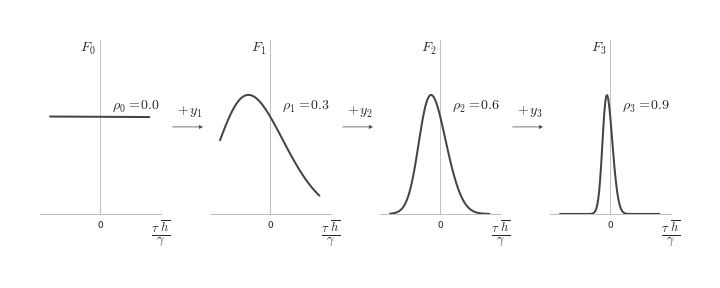
\includegraphics[scale=1.1]{modulation-function-rho.png}
\end{figure*}

\newcommand{\EF}{\ensuremath{\mathrm{F}(\,\htv\,|\gmt,\tau,\ns)}} O gradiente da função $\EV$ pode ser visto como uma \emph{força} que atua sobre $\wt$ na direção que aproxima o aluno do professor, composta pela direção $\tau\,\vec{x}$ e uma amplitude $F$. Chamaremos essa amplitude de \emph{Função de Modulação Bayesiana}, e para futuras referências
\begin{align}\label{eq:f-bayes}
    \EF & = - {\tau}\,\del{\htv} \EV = {\tau\gmt^2}\,\del{\htv}
    \ln\inbk{\ns-(1-2\ns)H\inpr{-\frac{\tau\htv}{\gmt}}} \notag \\ & =
    \frac{\gmt}{\sqrt{2\pi}}(1-2\ns)
    \frac{\exp\inbk{-\half\inpr{\frac{\htv}{\gmt}}^2}}{\ns + (1-2\ns)
      H\inpr{-\frac{\tau\htv}{\gmt}}}
\end{align}

É possível mostrar \footcite{Kinouchi1996,Vicente1998} que a grandeza $\gmt$ está relacionada com semelhança entre aluno e professor, dada por $\rho = \frac{\rl^T\wt}{||\rl||||\wt||}$, da seguinte forma
\begin{align}
    \gmt^2 & = \frac{1-\rho^2}{\rho^2}\label{eq:rho-def}
\end{align}
Essa relação facilita a compreensão da evolução de $\Ct$ ao longo do aprendizado, associando a adaptação na função de modulação diretamente ao desempenho do aluno condizente com os acertos relativos ao professor.
Tal adaptação da função de modulação pode ser descrita como um ajuste da relevância dada pelo aluno ao conteúdo dos exemplos de acordo com a experiência obtida até então.

Para compreender o que se passa, olhemos para a grandeza $\frac{\tau\htv}{\gmt}$.
O sinal de $\frac{\tau\htv}{\gmt}$ indica que o aluno classificou correta ou incorretamente o exemplo apresentado, enquanto seu valor absoluto indica o grau de \emph{surpresa/tédio} que o exemplo causa no aluno.
Essa interpretação vem do fato que $\tau=\pm 1$ e, portanto, $|\htv|$ indica quanta certeza o aluno tem em sua resposta, e portanto, um erro quando há muita certeza gera mais surpresa do que um acerto numa situação semelhante.  Ao longo do aprendizado, $\rho$ tende a aumentar, fazendo com que a função de modulação se adapte para dar mais relevância a exemplos que causem maiores surpresas.

A desconfiança do aluno sobre a classificação do professor, representada pela estimativa $\ns$ da probabilidade do professor estar errado, faz com que a função de modulação reduza a relevância de surpresas muito grandes, dando à função de modulação um caráter adaptativo.
Uma ilustração do comportamento da função de modulação em relação parâmetro $\rho$ e $\ns$ é dada pelas figuras \ref{fig:Frho} e \ref{fig:Fns}

\begin{figure*}[h!]\label{fig:Fns}
  \centering 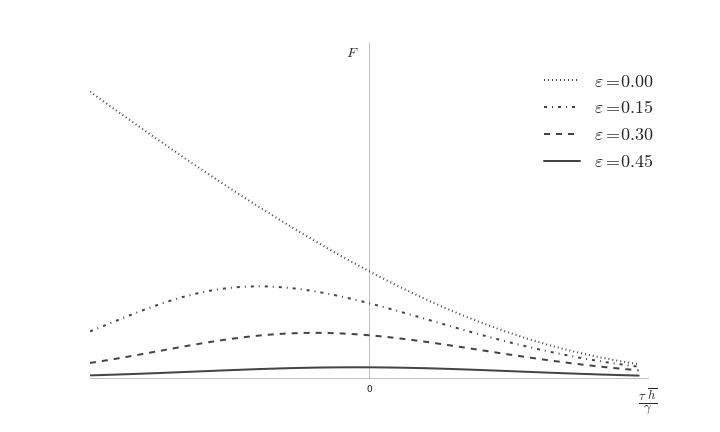
\includegraphics[scale=1.1]{modulation-function-eta.png}
  \caption{Comportamento da função de modulação $F$ com respeito ao aumento da desconfiança do aluno sobre possíveis erros do professor, para $\rho$ fixo. Valores de $\frac{\htv\tau}{\gmt}$ positivos ou negativos ocorrem quando o aluno classifica correta ou incorretamente o exemplo apresentado, o seu valor absoluto está associado com o grau de surpresa trazido pelo exemplo.}
\end{figure*}

Com base no cenário estabelecido, fica evidente que ao fixarmos um valor de $\rho$, fazendo com que a equação \eqref{eq:Ct-V} fique $\CT = \Ct$, a forma da função de modulação fica congelada.
Isso  é equivalente a fixar um algoritmo de aprendizado para o aluno que, na abordagem apresentada, é completamente determinado por $\rho$ e $\ns$.
A escolha de congelar a dinâmica para $\rho$, ao menos no que diz respeito à modelagem de comportamento humano, é motivada por estudos apontando que o desenvolvimento das áreas sociais do cérebro se desenvolvem no período da adolescência.
Nos estudos de \parencite{Choudhury2006, Blakemore2008,Moriguchi2007} é estabelecida, através de análises \emph{fMRI}, mudanças na atividade e na estrutura de áreas como o córtex pré-frontal, o córtex parietal e o córtex temporal superior, associados com o desenvolvimento da cognição social.
Neste trabalho, teremos sempre fixado um valor de $\rho$, sinalizando que a estratégia de aprendizado dos agentes foi previamente estabelecida, numa analogia com agentes \emph{``adultos''} do ponto de vista de cognição social.

A dedução acima foi feita com base na teoria de aprendizado de máquina e deixou de fora vários aspectos interessantes desse campo de estudo.
Leitores interessados no assunto podem consultar \parencite{Engel2001, Hastie1993} para abordagem completa e \parencite{Kinouchi1996, Solla1999,Opper1996} para aprofundar os conceitos apresentados nessa seção.

\subsection{Um Modelo mais Simples de Aprendizado}
\label{ssec:SLM}

A dedução acima nos proporciona um algoritmo de aprendizado supervisionado que maximiza o aprendizado por exemplo apresentado, mas essa vantagem é obtida pelo preço da interpretação do algoritmo, dificultada pela forma não muito amigável da função de modulação \eqref{eq:f-bayes}.
Para tentar sanar esse problema, vamos abstrair as características da função de modulação ótima e tentar criar uma forma mais simples que as mantenha.

Primeiramente, note que a equação \eqref{eq:f-bayes} como função da variável que mede $\frac{-\tau\,h}{\gmt}$ a concordância entre as respostas do aluno e do professor pode ser vista como uma atribuição de pesos para cada grau de concordância.
Em outras palavras, a função de modulação é responsável pela diferença na relevância dada a exemplos que corroboram a classificação do aluno e aqueles que o surpreendem, com $\frac{-\tau\,h}{\gmt}$ respectivamente positivos e negativos.
Essa é a principal característica dos algoritmos de aprendizado e, portanto, a principal forma de caracterizá-los.
Por exemplo, os algoritmos tradicionais como o de \emph{Hebb} ou o \emph{Perceptron} tem como única distinção o fato do primeiro dar mesmo valor a todos os exemplos e o segundo dar valor apenas aos que trazem novidade, que surpreendem.

No presente contexto, a forma de ajustar a relevância dada à exemplos com carga corroborativa ou surpreendente é fixando os valores do estilo cognitivo $\rho$ e da desconfiança $\ns$.
Podemos pensar uma forma simplificada, $F_{MF}$, para a função de modulação \eqref{eq:f-bayes} que tenha essas características de regular o peso entre corroboração e novidade através dos parâmetros $\rho$ e $\ns$.
Será útil também definir um custo cognitivo simplificado, $V_{MF}$, associado ao erro na classificação.

\newcommand{\EFmf}{\ensuremath{F_{MF}}}
\newcommand{\EVmf}{\ensuremath{V_{MF}}}
% A função de modulação \eqref{eq:f-bayes} é relativamente complicada, tornando impraticável o desenvolvimento analítico do modelos de mecânica estatística que serão desenvolvidos a seguir.
% Será útil, portanto, definir uma função de modulação mais tratável e que mantenha algumas das características descritas da equação \eqref{eq:f-bayes}.
% Em particular, vamos fazer com que a nova função que reproduza o comportamento da função de modulação relativo à diferença de relevância dada à exemplos corroborativos e novidades, bem como a possível regulação de absurdos.
% Através dessa nova função, que chamaremos $\EFmf$, podemos obter uma energia associada ao erro de classificação, à qual chamaremos $\EVmf$, definidos da seguinte forma
\begin{align}
    \EFmf(z|\,\rho,\ns,z_0) & = \frac{1-\rho}{2}
    - \frac{\rho}{2}\sgn(z)
    + \half\sgn(z+z_0) \label{eq:f-mf} \\[4pt]
    \EVmf(z|\,\rho,\ns,z_0) & = - \frac{1-\rho}{2}z
    + \frac{\rho}{2}|z| -
    \half|z+z_0| \label{eq:v-mf}
\end{align}
onde as grandezas $z$ e $z_0$ estão relacionadas com o parâmetro de concordância $\frac{-\tau\,h}{\gmt}$.

Para entender as grandezas $z$ e $z_0$, vamos olhar para o gráfico da funções \eqref{eq:f-mf}, ilustrado na figura \ref{fig:mf-func}, e associá-las às características descritas acima.
\begin{figure}[h!]\label{fig:mf-func}
    \centering
    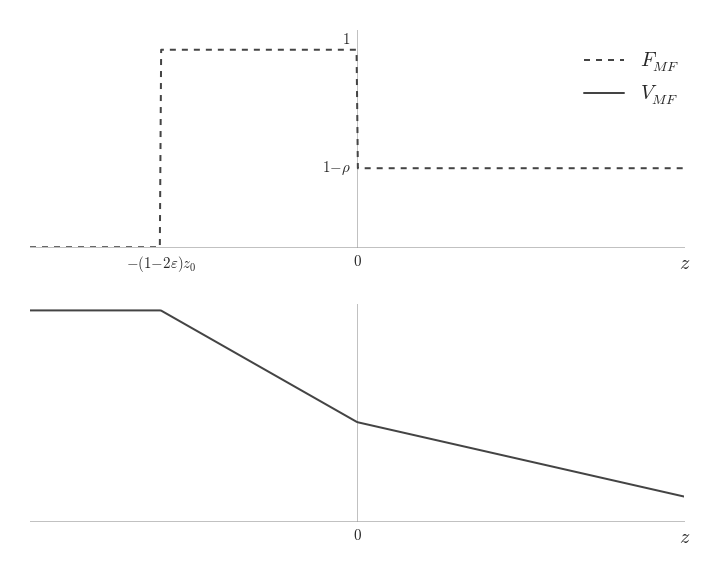
\includegraphics[scale=0.5]{mean-field.png}
    \caption{Ilustração das função aproximadas $\EFmf$ e $\EVmf$}
\end{figure}

Como discutido acima, $F_{MF}$ regula a relevância entre óbvio e novidade, logo $z$ deve ser uma função de $\frac{-\tau\,h}{\gmt}$.
O parâmetro $z_0$ é um valor de discordância que indica um conflito tão grande com o conhecimento do aluno que o faz ignorar a resposta do professor, ou seja é o ponto a partir do qual o aluno considera a informação daquele exemplo como \emph{'besteira'} e não o absorve.
É evidente, olhando para a função de modulação Bayesiana \eqref{eq:f-bayes}, que $z_0$ deve ser uma função de $\ns$ e $\rho$.

Para determinar o comportamento de $z_0$, basta otimizar o erro quadrático entre $F_{MF}$ e $F$ em relação ao valor de $z$, que levará ao valor $z=z_0$ para o qual $F$ tem a metade da altura máxima.
Alternativamente, é possível considerar $z_0$ como um grau de liberdade a mais no modelo e estudar sua influência no comportamento do campo médio.

% \vfill
\section{Modelos de Agentes e Mecânica Estatística}
\label{sec:AMSM}

\subsection{Estabelecendo a Linguagem do Modelo de Agentes}\label{ssec:AMSM1}
A hipótese central deste estudo de fenômenos sociais é que as propriedades de uma sociedade surgem da interação entre os indivíduos que a integram.
Essa forma de abordar o problema tem a vantagem de requerer apenas a compreensão do que é um indivíduo e como ele atua com outros semelhantes a ele, ou seja, é necessária apenas uma compreensão local do sistema para inferir algumas características globais.
É claro que essa estratégia pode ser criticada por um excesso de simplificação ao desconsiderar características particulares, tanto no que diz respeito ao indivíduo quanto a suas relações.
Entretanto, é necessário ter em mente que o objetivo não é detalhar o resultado de cada interação possível entre indivíduos, mas sim tentar reproduzir o comportamento macroscópico que observamos em diversas culturas e, se possível, sua relação com aspectos intrínsecos da natureza humana.

\newcommand{\agt}[1]{\ensuremath{\vec{w}_{#1}}}
\newcommand{\vrt}{\ensuremath{\mathcal{V}}}
\newcommand{\edg}{\ensuremath{\mathcal{E}}}
\newcommand{\MM}{\ensuremath{\mathcal{W}}}
Para elaborar um modelo de agentes capaz de descrever fenômenos sociais atribuídos a cultura, moral ou estratégias políticas, entre outros fenômenos relacionados a comportamento aprendido, precisamos entender ou, no mínimo emular, como se dá o processo de aprendizado social.
Considere um conjunto de vértices $\vrt = \{1,\dots,N\}$ e um conjunto de vetores $\MM = \{\agt{i} | i \in \vrt \}$, representando \emph{agentes} que interagem através da troca de informações e aprendem uns com os outros, de acordo com a estrutura das \emph{relações sociais} estabelecidas em $\edg \subset \vrt \times \vrt$ denotando $(ij)\in\edg$ quando os agentes $i$ e $j$ são parceiro sociais \footnote{Note que as relações estabelecidas em $\edg$ não são, necessariamente, simétricas.
É possível que um agente considere outro um parceiro sem   reciprocidade}.
Cada agente é representado por vetor $\agt{i} \in \R^K$ que representa sua experiência \footnote{num contexto determinado pelo fenômeno social em estudo} e um índice $i \in \vrt$, e pode receber a \emph{opinião} de um agente com quem se relaciona sobre um \emph{assunto} ou \emph{questão} $\vec{x} \in \R^K$ que tem alguma relação semântica com os vetores $\vec{w}$.

\newcommand{\cogcost}{\ensuremath{{\mathrm{V}}}}
\newcommand{\opn}[3][1]{\ensuremath{
      {#1\over \sqrt{K}} \agt{#2} \cdot \vec{#3}}}
\newcommand{\cost}{\ensuremath{{\mathcal{H}}}}
\newcommand{\SG}{\ensuremath{\mathcal{G}}}
\newcommand{\soc}{\ensuremath{\mathcal{S}}}
A interação entre dois agentes é regulada pelo custo cognitivo $\cogcost$, atribuído ao processo de aprendizado da \emph{opinião} $h = \opn{ }{x}$ de um agente pelo outro.
Considerando a soma do custo cognitivo sobre todos os pares de agentes no grafo temos o custo social total
\begin{align}
  \cost = \sum_{(i,j)\in \edg} J_{ij} \cogcost_{ij} \label{eq:Scost}
\end{align}
Chamaremos de \emph{Sociedade de Agentes}, ou apenas \emph{sociedade}, ao conjunto $\soc = (\SG, \MM, \cost)$, onde $\SG = (\vrt,\edg)$ é o grafo das interações sociais.

A natureza dos vetores $\MM$ depende do fenômenos em estudo.
No caso de aprendizado moral, como em \parencite{Cesar2014, Vicente2014}, o vetor $\agt{i}$ representa a matriz moral do agente $i$, e o processo de aprendizado entre os agentes pode levar ou não a um consenso sobre como é o comportamento \emph{ético} daquela sociedade.
Por outro lado, numa escala mais ampla, como no modelo em \parencite{Axelrod1997}, os vetores $\MM$ podem representar características culturais de agrupamentos de pessoas, cenário no qual cada agente representa, digamos, uma vila e a troca de características culturais entre agentes representa a dinâmica de estruturas culturais, possibilitando o surgimento de fronteiras isolando diferentes culturas que, de alguma forma, se tornaram \emph{incompatíveis}.

A topologia do grafo social, em particular o número de parceiros sociais, tem uma grande influência na possibilidade da sociedade experimentar uma transição de fases.
Somado a isso, o fato das estruturas sociais dependerem da dinâmica entre os indivíduos cria uma dinâmica para as relações entre agentes.
Esse efeito mútuo da influência do grafo nas características do indivíduo e vice-versa deve ser contemplado pelo modelo.
Para isso, introduzimos a matriz de adjacência das relações sociais, com elementos $R_{ij}$.
Estabeleceremos uma dinâmica para as relações sociais de modo que os valores de $R_{ij}$ estejam entre $0$ e $1$, se anulando quando os agentes $i$ e $j$ deixam de interagir, ou seja quando $(ij) \notin \soc$.
% \begin{equation}
%  R_{ij} =
%   \begin{cases}
%     0 < R \leq 1, & \text{ se } (ij) \in \edg \\
%     0, & \text{ caso contrário}
%   \end{cases}
% \end{equation}

A determinação da função custo cognitivo está relacionada com a dinâmica de aprendizado supervisionado desenvolvido na seção \ref{sec:ML} através de uma analogia. Cada agente na sociedade pode desempenhar tanto o papel de \emph{ aluno} quanto o de \emph{professor}.
Essa alternância de papeis é interpretada como uma sequência de diálogos entre agentes, nos quais ora um agente expressa sua opinião sobre uma questão, ora recebe a opinião de algum parceiro social.
Na situação em que a opinião de um colega é recebida, o agente se comporta como um aluno, tentando aprender a reproduzir o comportamento do outro agente. \footnote{É possível impor um comportamento antagonista, no qual um agente ativamente caminha no sentido oposto ao colega locutor.
A analogia se mantém considerando que o professor seria um agente com a orientação oposta à do agente que expressa a opinião.}

Com base nas equações \eqref{eq:wt-V}, \eqref{eq:Ct-V} e \eqref{eq:Vh}, podemos estabelecer um \emph{evento} envolvendo os parceiros sociais $(ij) \in \edg$ como uma relação \emph{aluno/professor} na qual $i$ aprende a opinião $h_j = \opn{j}{\vec{x}}$ do agente $j$ a respeito de um assunto $\vec{x}$.
O desempenho de $i$ com relação a essa tarefa é estimada pelo custo cognitivo $\cogcost_{ij}(\vec{x}) = V(\agt{i},\agt{j},\vec{x})$.

Como argumentado em \parencite{Cesar2014}, pessoas passam por diferentes estágios de aprendizado ao longo vida.
Quando mais  jovens, as estratégias de aprendizado social estão se formando, e podemos associar a resposta de uma criança ao se defrontar com diversos exemplos com a evolução da função de modulação ilustrada na figura \ref{fig:Frho}.
Ao passo que novidade é encontrada, a criança altera, de forma inconsciente, a relevância relativa dada a exemplos surpreendentes ou corroborativos.
Entretanto, após uma certa idade o modo como as pessoas aprendem fica \emph{`congelado`}, sendo associado a um algoritmo de aprendizado fixo no contexto de aprendizado de máquinas.
Em termos das equações da dinâmica de aprendizado \eqref{eq:wt-V} e \eqref{eq:Ct-V}, isso equivale à fazer $\gmt_i$ constante, e por consequência $\rho_i$ constante. Desse modo, fixando $\rho_i$, nossa analogia trata de agentes \emph{`adultos`} no aspecto de aprendizado social.
Com base nos argumentos dados em \parencite{Caticha2011}, a tendência de associação entre indivíduos mais parecidos nos estimula a fixar um único $\rho$ para grupos de agentes parceiros ou mesmo para toda uma sociedade.
\newcommand{\Vab}[2]{\ensuremath{\cogcost_{#1#2}}}
\newcommand{\gm}{\ensuremath{\gamma}}
\newcommand{\stb}{\ensuremath{\frac{\tau_j h_i}{\gm}}}
Com essas considerações, podemos escrever um custo cognitivo e a função de modulação para um evento entre os parceiros $i$ e $j$ da seguinte maneira
\begin{align}
    \Vab{i}{j}(\vec{x}) & = -\gm^2\ln\inbk{\ns
      + (1-2\ns)H\inpr{-\stb}} \label{eq:Vij}  \\[4pt]
    F_{ij}(\vec{x}) & = \frac{\gm(1 - 2\ns)}{\sqrt{2\pi}}
    \frac{\exp\inbk{-\half\inpr{\frac{h_i}{\gm}}^2}}{\ns
      + (1-2\ns)H\inpr{-\stb}} \label{eq:Fij}
\end{align}
onde $\tau_j = \sgn(h_j)$ e $\gm^2 = \frac{1-\rho^2}{\rho^2}$.

O parâmetro $\ns$, introduzido no contexto do aprendizado de máquina como uma estimativa do aluno para a probabilidade de receber uma informações equivocadas do professor, desempenha o papel de uma \emph{desconfiança} no contexto de aprendizado social, possibilitando a rejeição de opiniões muito dissonantes.
A interpretação da informação trazida por exemplos através de surpresa ou corroboração para o aluno no cenário do aprendizado de máquina é traduzido no contexto de aprendizado social para uma dicotomia entre \emph{concordância} e \emph{discordância} das opiniões.
Dessa forma, fica clara uma interpretação do custo cognitivo como um preço a ser pago pela discordância entre dois agentes e o custo social, $\cost$, como uma energia necessária para sustentar uma sociedade com um certo grau de diversidade nas opiniões dos agentes.

É evidente, pela forma do potencial $\Vab{i}{j}$, que embora opiniões \emph{`absurdas`} do agente $j$ sejam ignoradas pelo agente $i$, o mínimo global de $\cost$ estará mais próximo do estados de $\MM$ que desempenham o maior valor possível de concordância entre todos os agentes, caracterizando um consenso global quando o agentes trocam informação sobre uma questão apenas, como verificado em  \parencite{Caticha2011}.

Para sustentar a coexistência de diversidade entre agentes com as mesmas características cognitivas, a saber $\rho$ e $\ns$, é necessário criar um mecanismo que reduz o custo pago em presença de discordância, aliviando a pressão social.
Isso é feito dando a cada agente o poder de construir ou destruir suas relações sociais por meio das opiniões recebidas, através do controle das relações sociais $R_{ij}$.
A dinâmica das relações sociais é definida da seguinte forma
\begin{align}
  R_{ij}^{+} & = (1-\varphi)R_{ij} + \lambda R_{ij}(1 - R_{ij})\sgn(h_ih_j) \label{eq:Rt}
\end{align}
onde $R_{ij}^{+}$ é a relação entre $i$ e $j$ após um evento de interação, $\lambda$ um parâmetro que controla a \emph{`euforia`} no ajuste da relação e $\varphi$ um parâmetro que controla o \emph{`esquecimento`} dessa relação. A grandeza $J_{ij}=J(R_{ij})$ que aparece na equação \eqref{eq:Scost} está relacionada, de alguma forma a ser escolhida de acordo com o contexto específico do fenômeno estudado,com as relações sociais $R_{ij}$ e tornará possível a regulação do comportamento de aproximação ou rejeição relativo a uma opinião.
Note que as relações sociais se intensificam caso os agentes concordem num evento e são reduzidas caso contrário, fazendo o papel de uma espécie de registro da taxa de concordância do agente $i$ com as opiniões do agente $j$.

\subsection{Mecânica Estatística de Sistemas Sociais}\label{ssec:AMSM2}

Do que foi discutido na elaboração da linguagem que usaremos ao lidar com fenômenos sociais, ficam claros dois pontos importantes do modelo: sua natureza estatística e a importância delegada ao custo social, $\cost$.
Para avançar, faremos uso de métodos típicos da mecânica estatística, possibilitando a compreensão de alguns termos usado de forma vaga anteriormente, como \emph{`consenso`} ou \emph{`pressão`} e providenciando algumas previsões de comportamento do modelo.

Primeiramente, vamos determinar a probabilidade $P(\MM)$ de termos
uma sociedade $\soc = (\MM, \SG, \cost)$ num determinado estado $\MM$ com uma configuração social $\SG$ fixa.
Dos argumentos apresentados, somos levados a esperar algum valor para a função custo, ou seja devemos ter $P(\MM)$ tal que $\langle\cost\rangle=E \in \R$, onde $\langle\dots\rangle$ denota o valor esperado sobre $P(\MM)$.
Embora não tenhamos o valor $E$ para cada estado, essa expectativa indica nosso interesse na avaliação da função $\cost$.

A determinação de $P(\MM)$ é feita através da maximização da entropia relativa dela com alguma à priori $Q(\MM)$, que tomamos como uma distribuição uniforme em $\MM$ \footnote{Essa escolha é guiada pelo princípio da máxima ignorância e pelo fato da distribuição à priori carregar o mínimo de informação a respeito de um conjunto de variáveis, a saber apenas os possíveis valores que elas podem tomar.}, sujeita ao vínculo de valor esperado do custo social.
A entropia relativa entre $P$ e $Q$ é dada por
\begin{align}\label{eq:ent-Pw}
  S[P(\MM):Q(\MM)] & = -\int \msr{\MM} P(\MM) \ln \frac{P(\MM)}{Q(\MM)} \notag \\
                   & \quad + \beta \inbk{E - \int \msr{\MM} P(\MM)\cost}
\end{align}

Igualando a zero derivada funcional de $S$ relativa a $P$, notando que $Q$ é uma constante, obtemos a forma da distribuição $P$ que maximiza a entropia, a saber a distribuição de \emph{Boltzmann}, dada por
\begin{align}
  P(\MM) & = \frac{1}{Z} \exp (-\beta \cost [\MM]) \label{eq:Pw} \\
\intertext{onde $Z$ é a função de partição}
  Z & = \int \msr{\MM} \exp (-\beta \cost [\MM]) \label{eq:Zw}
\end{align}

O parâmetro $\beta$, introduzido como um multiplicador de \emph{Lagrange} associado ao vínculo do valor esperado do custo social, pode ser interpretado analisando a distribuição $P$ obtida.
Note que, supondo um valor fixo de $\beta \neq 0$, estados com custos sociais mais elevados se tornam menos prováveis de acordo com $P(\MM)$.
Isso implica que a evolução da sociedade sobre a dinâmica definida por $\cost$ deve seguir na direção de reduzir os custos sociais. Neste caso, $\beta$ é uma espécie de \emph{pressão}, determinando a escala de flutuações do custo social relativo ao valor esperado $E$.

A natureza da pressão $\beta$ depende em parte do contexto, embora seja claro que ela está relacionada com a pressão sobre cada agente perante a exibição de um comportamento \emph{`transgressor`} relativo a seus parceiros, e por esse motivo a chamaremos de \emph{pressão social} \footnote{No contexto de concorrência partidária, daremos um nome mais sugestivo para a pressão, mas por enquanto, pressão social é suficiente para o entendimento do que segue.}.
Essa interpretação nos leva a crer que, fixadas as relações sociais, ou seja fazendo $R_{ij}$ constantes, e dada suficiente pressão encontraremos a sociedade apenas em estados de \emph{consenso} de opinião a respeito da questão colocada.
Para testar essa intuição, seguiremos com um estudo de campo médio visando estabelecer as condições em que tal situação de consenso pode ocorrer.

\newcommand{\qst}{\ensuremath{\vec{x}}}
\newcommand{\cutoff}{\ensuremath{\eta}}
Considere uma sociedade $\soc_0=(\MM,\SG,\cost_0)$, com as relações sociais $\SG$ fixadas a função custo social $\cost_0 = \sum J_{ij} V^0_{ij}$ com
\begin{align}\label{eq:V0ij}
  V^0_{ij} & = -\frac{1-\rho}{2}h_ih_j +\frac{\rho}{2}|h_ih_j|
               - \half|h_ih_j + \cutoff|
\end{align}
uma aproximação do custo cognitivo, como destacado na seção \ref{sec:ML} com a equação \eqref{eq:v-mf}. Os agentes são descritos por vetores $\agt{i}\in\R^K$ e trocam opiniões sobre um único assunto $\qst\in\R^K$.
Vamos supor que $|\agt{i}|^2=|\qst|^2=K$ para todo $i$ e chamar $h_i = \opn{i}{\qst}$, de modo que $-\sqrt{K} \leq h_i \leq \sqrt{K}$ e $\cutoff = (1-2\ns)K$.
Essa escolha para o valor de $\cutoff$ está relacionada com o parâmetro $z_0$ comentado na seção \ref{ssec:SLM}, tratando-o como um grau de liberdade extra, e pode ser encarada como um modelo para o comportamento de $\cutoff$ em termos de $\ns$.
Como veremos, a influência de $\cutoff$ para um valor linear em $\ns$ não afeta as fases observadas no campo médio, dissonando do resultado obtido para o potencial Bayesiano.

Para possibilitar o tratamento da função de partição \eqref{eq:Zw}, além da introdução do potencial $V^0$, vamos supor que os $J$ são distribuídos de forma homogênea em $\SG$, ou seja
\begin{equation*}
  J_{ij} = \begin{cases}
    J_0 > 0 & \text{se $i$ e $j$ são parceiros sociais} \\
    0 & \text{caso contrário}
    \end{cases}
\end{equation*}
e que $\SG$ é um grafo regular não direcionado, o que significa que cada agente tem o mesmo número $n_0$ de parceiros e todas as relações são recíprocas.
\footnote[][-7cm]{Essa hipótese é bem restritiva, mas não é artificial, dado que grafos sociais frequentemente apresentam uma estrutura quase regular como grafos de \emph{mundo pequeno}, onde o grau médio de cada vértice é representativo globalmente.
Esse pode não ser o caso em estruturas mais assimétricas como  grafos de \emph{Barabasi-Albert}.
Mas em se tratando do campo médio, a estrutura do grafo seria descartada de todo modo, então essas consideração servem apenas para indicar as situações em que os resultados simulados ou experimentais não podem ser explicado apenas pela aproximação de campo médio.}

Com essas hipóteses adicionais, podemos nos questionar qual é a distribuição $P_* = \prod_i^N P_i$, sujeita ao vínculo do valor esperado do custo social, que melhor aproxima a distribuição $P(\MM)$ por um sistema de agentes independentes?
Para responder essa pergunta, usamos mais uma vez a maximização da entropia em relação às distribuições $P_i$.
A entropia relativa entre $P$ e $P_*$ é
\begin{align}
  S[P_*:P] & = -\int \msr{\MM} P_* \ln \frac{P_*}{P}
               + \beta\inbk{E - \int\msr{\MM}P_*\cost} \notag\\
           & = -\sum_j^N\int\msr{\agt{j}}P_j\ln {P_j \over P}
               \notag\\
           & \quad + \beta\inbk{E-\sum_{(kj)\in\SG}\int
                 \msr{\agt{k}}\msr{\agt{j}}P_kP_jJ_0V^0_{kj}}
               \label{eq:ent-P*}
\end{align}
onde usamos implicitamente a normalização de cada $P_j$.
Tomando a derivada funcional de S em relação a $P_i$ e igualando a zero teremos, usando o fato de $P$ e $E$ serem independentes de $P_i$
\begin{align}
   0 = {\delta S \over \delta P_i} & = 1 - \ln P_i -\beta J_0\sum_{j\in n(i)}\int\msr{\agt{j}}P_jV^0_{ij} \notag\\
  \Rightarrow P_i & = \frac{1}{Z_i}\exp\inbk{-\beta J_0 \sum_{j\in n(i)}\int \msr{\agt{j}}P_j V^0{ij}} \label{eq:PiV}
\end{align}
denotando por $n(i) = \{j | (ij)\in \SG \}$ o conjunto dos parceiros sociais do agente $i$.

Para prosseguir, será necessário trabalhar com a integral
\begin{align}
  I_i & = \int \msr{\agt{j}}P_j V^0_{ij} \notag\\
      & = \int \msr{\agt{j}}P_j \inbk{-h_ih_j + \frac{\rho}{2}|h_ih_j| - \half|h_ih_j+\cutoff|} \label{eq:lnPiV}
\end{align}
que aparece no lado direito da equação \eqref{eq:PiV}.
Somente nesse ponto a escolha do custo cognitivo \eqref{eq:V0ij} se justifica, tendo em vista que mesmo a definição dos parâmetros de ordem, no que seguirá, seria mais difícil, senão impossível, com o potencial \eqref{eq:Vij}.
Note também que, o potencial \eqref{eq:V0ij} é uma forma um pouco mais geral daquele usado em \parencite{Caticha2011}, se reduzindo àquele no caso em que a desconfiança é nula, ou seja $\ns = 0$.
De fato, a análise de campo médio apresentada aqui segue os moldes da estabelecida em \parencite{Caticha2011,Cesar2014}.

Para determinar a distribuição $P_i$, definimos os parâmetros de ordem
\begin{align}
  m & = \int \msr{\agt{j}} P_j \opn{j}{\qst} \label{eq:m-def} \\
  r & = \int \msr{\agt{j}} P_j \left|\opn{j}{\qst}\right| \label{eq:r-def}\\
\intertext{e substitua em \eqref{eq:lnPiV} para obter}
  I_i & = -m{1-\rho \over 2 \sqrt{K}}\agt{i}\cdot\qst
          +r\,\frac{\rho}{2\sqrt{K}}\left|\agt{i}\cdot\qst\right|
          - {1\over 2 \sqrt{K}}\left|m\,\agt{i}\cdot\qst+\cutoff\right| \label{eq:Ii}
\end{align}
Note que assumimos a homogeneidade dos parâmetros de ordem, ou seja, fizemos $m_j = m$ e $r_j = r$ para todo $j$.
Isso não  significa que os são idênticos, mas que são descritos de forma idêntica.
Essa hipótese está relacionada com a homogeneidade das relações, explicitada pela constante $J_0$.
Fizemos também a escolha de comutar a integral com o valor absoluto no termo que envolve a desconfiança para facilitar as contas e por manter a coerência, mas sem uma justificativa formal para isso.
Substituindo \eqref{eq:Ii} em \eqref{eq:PiV} e lembrando que todos agentes têm o mesmo número de parceiros $n_0$, chegamos à conclusão
\begin{align}
  P_i & = \frac{1}{Z_i}\EulerE^{-\beta\,J_0\,n_0\,I_i} \label{eq:Piw}
\end{align}

O resultado obtido para as probabilidade $P_i$ nos traz um conjunto de equações que precisam ser resolvidas de forma autoconsciente, a saber
\begin{align}
  m & = \frac{1}{Z} \int \msr{\agt{i}} \inpr{\opn{i}{\qst}}\EulerE^{-\beta\,J_0\,n_0\,I_i(m,r)} \label{eq:sc-m}\\
  r & = \frac{1}{Z} \int \msr{\agt{i}} \left|\opn{i}{\qst}\right|\EulerE^{-\beta\,J_0\,n_0\,I_i(m,r)} \label{eq:sc-r}\\
  Z & = \int \msr{\agt{i}}\EulerE^{-\beta\,J_0\,n_0\,I_i(m,r)} \label{eq:sc-Z}
\end{align}
A solução desse sistema de equações resulta na determinação das distribuições $P_i$ para todo os agentes, e por consequência determina nossa aproximação de campo médio.
Entretanto, a equação \eqref{eq:Piw} nos dá a probabilidade $P_i = P(\agt{i})$ de encontrar um agente com um estado interno $\agt{i}$ do agente.
Essa situação é inconveniente por dois motivos, a saber, por não termos acesso direto ao estado cognitivo das pessoas nos processos formadores de opinião e, também, por estarmos interessados, de fato, nas opiniões.
Para resolver esse conflito entre o resultado \eqref{eq:Piw} e sua praticidade, façamos
\begin{align}
  P(h) & = \int \msr{\agt{ }} \delta\inpr{h - \opn{ }{\qst}} P(\agt{ }) \notag \\[4pt]
       & = \frac{1}{C}(1 - h^2)\,\EulerE^{\,\beta J_0 n_0 \inbk {
         \frac{1-\rho}{2}hm - \frac{\rho}{2}|h|r + \half|hr + \cutoff|}} \label{eq:Ph}\\
\intertext{com a nova função de partição $C$ dada por}
  C & = \int _{-\sqrt{K}}^{\sqrt{K}} \msr{t} (1 - t^2)\,\EulerE^{\,\beta J_0 n_0\inbk{
       \frac{1-\rho}{2} mt - \frac{\rho}{2}r|t| + \half|rt + \cutoff|}} \label{eq:Zh}
\end{align}

Os parâmetros ordem $m$ e $r$ são os valores esperados das opiniões e das suas \emph{`convicções`} sobre $\qst$ em toda a sociedade.
Com isso podemos estudar as condições definidas pela pressão social $\beta$, pelo estilo cognitivo $\rho$ e pela desconfiança $\ns$ na formação de consenso através dos valores dos parâmetros de ordem. O comportamento típico do parâmetro $m$, que mede a média das opiniões em relação à questão dada, está ilustrado na figura \ref{fig:pd-ferro}.

\begin{figure}[h!]\label{fig:pd-ferro}
  \centering
  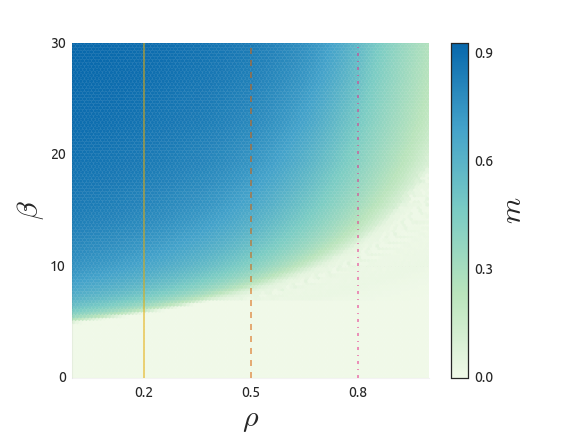
\includegraphics[scale=1.0]{phase-diagram-ferro.png}
  \caption{Diagrama de fases da solução $m$ das equações de campo médio, no plano $\beta \times \rho$.
Esse comportamento não se altera para baixos valores da desconfiança $\ns$ neste cenário de agentes similares em estratégia de aprendizado e motivados a cooperar.}
\end{figure}
\begin{marginfigure}[-7cm]
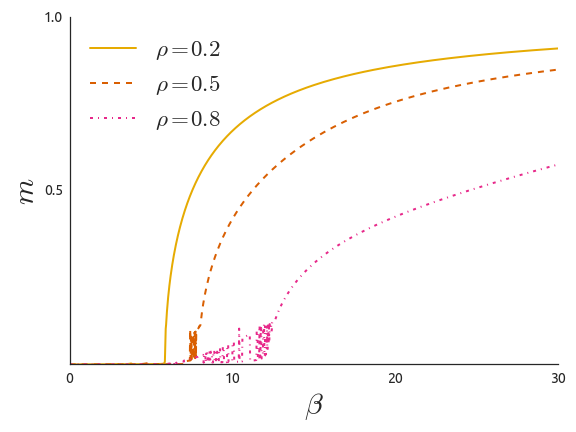
\includegraphics[scale=1.5]{m-curves-ferro.png}
\caption{Curvas de consenso correspondentes às retas verticais na figura \ref{fig:pd-ferro}.}
\end{marginfigure}

A figura \ref{fig:pd-ferro} mostra que, seguindo uma das linhas verticais que fixa um valor de $\rho$, há uma transição de fase entre os estados de dissenso e consenso com relação às opiniões dos agentes a respeito da questão $\qst$.
Sem se desprender do contexto, no cenário em que a concordância é estimulada, dado o parâmetro $J_0 > 0$, existirá uma pressão social crítica que levará essa sociedade ao consenso.
Esse tipo de comportamento é que esperamos dentro de um grupo com alguma ideologia ou de agentes que compartilhem um certo conjunto de características não muito disperso, codificado nos vetores $\agt{i}$.
Analogamente, situações onde a concordância seja muito relevante, talvez em condições de perigo à sociedade, é de se esperar que a sociedade atinja o consenso em detrimento da manutenção de diferenças.

Note, porém que maiores valores de $\rho$ tendem a apresentar pressões críticas mais elevadas.
Podemos imaginar numa sociedade com diferentes valores de $\rho$ a possibilidade de parte dos agentes estarem sob suficiente pressão social para obter consenso, mas outra parte não.
Logo, a analogia com ameças à sociedade nos levaria a associar essa variação às diferenças no que os agentes consideram ameaça ou não.
Essa aparente dicotomia sugere uma relação entre os comportamentos liberal e conservador exibido pelas pessoas e uma análise mais detalhada dessa relação pode ser encontrada em \parencite{Caticha2011,Vicente2014,Cesar2014}.

\begin{figure}[t!]\label{fig:pd-ferro-eps}
  \centering
  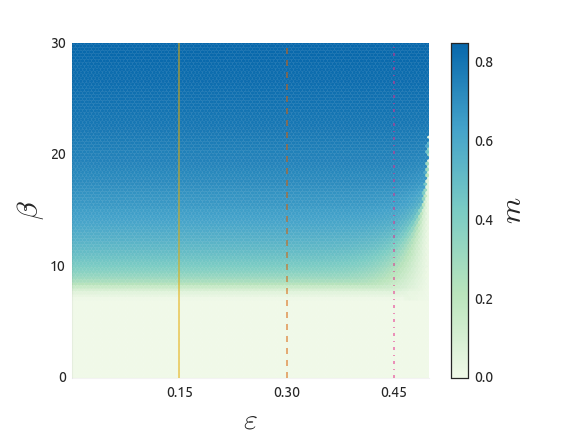
\includegraphics[scale=1.0]{eps-phase-diagram-ferro.png}
  \caption{Diagrama de fases da solução $m$ das equações de campo médio, no plano $\beta \times \varepsilon$.
Note como apenas valores de $\ns$ próximos de $0.5$ introduzem dificuldades ao surgimento de consenso.
Isso significa que, em campo médio, apenas sociedade em que quase nenhuma confiança pode ser atribuída aos parceiros é possível impedir o consenso.}
\end{figure}
\begin{marginfigure}[-9cm]
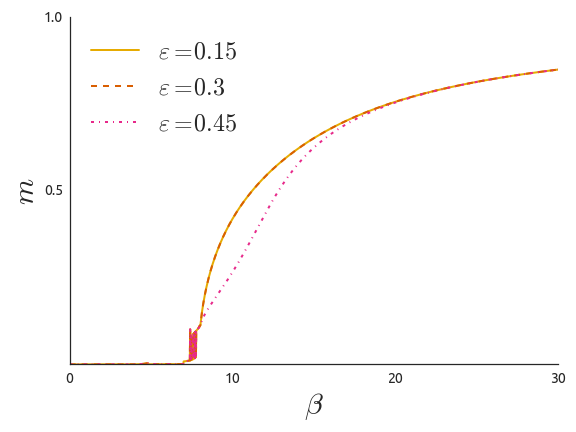
\includegraphics[scale=1.5]{eps-m-curves-ferro.png}
\caption{Curvas de consenso correspondentes às retas verticais na figura \ref{fig:pd-ferro-eps}.}
\end{marginfigure}

Uma propriedade interessante desse resultado é sua robustez perante mudanças na desconfiança $\ns$, como pode ser visto na figura \ref{fig:pd-ferro-eps}.
Essa condição nos diz relações internas de algum segmento social tendem a atingir consenso, mesmo com pouca confiança nas opiniões dos parceiros.
Tendo em vista a diversidade de opiniões relativas a um dado assunto, essa conclusão é de fato irreal.
O caso é que fixadas as relações sociais, a pressão dos pares eventualmente conduz ao consenso numa \emph{`vitória`} por resistência.

Vejamos um cenário em que uma sociedade tem dois grupos \emph{`rivais`} coexistindo.
Nessa situação, cada agente $i$ pode integrar um grupo $A=\{1,\dots,N_A\}$ ou um grupo $B=\{1,\dots,N_B\}$.
O custo cognitivo da interação entre os quaisquer dois agentes $(ij)$ é dado pela equação \eqref{eq:V0ij}, porem as grandezas $J_{ij}$ que regulam as interações sociais dependem dos grupo de $i$ e $j$.
Considere
\begin{align}\label{eq:J-antiferro}
  J_{ij} =
  \begin{cases}
    1 & \text{se $i$ e $j$ estão no mesmo grupo} \\
    -J & \text{com $J > 0$ caso contrário}
  \end{cases}
\end{align}
de modo que o custo social pode ser escrito
\begin{align}
  \cost_{AB} & = \sum_{\substack{i\in A\\j \in A}} V^0_{ij}
  + \sum_{\substack{i\in B\\j \in B}} V^0_{ij}
  - J\sum_{\substack{i\in A\\j \in B}} V^0_{ij} \label{eq:H-antiferro}
\end{align}
e podemos aplicar uma aproximação de campo médio análoga à feita para o cenário anterior.

Vamos aproximar a distribuição de \emph{Boltzmann} para a sociedade com custo social $\cost_{AB}$ por uma distribuição $P_{AB}=\prod_{i\in A}P_A(\agt{i})\prod_{j\in B}P_B(\agt{j})$, novamente através da maximização da entropia.
Seguindo essa estratégia, obteremos as seguinte formas para $P_A(\agt{i})$ e $P_B(\agt{j})$
\begin{align}
  P_A(\agt{i}) & \propto \EulerE^ {-\beta I_A(\agt{i})} \label{eq:PA}\\
  P_B(\agt{j}) & \propto \EulerE^ {-\beta I_B(\agt{j})} \label{eq:PB} \\
\intertext{com os termos $I_A$ e $I_B$ dados por}
  I_A(h_i) & = \sum_{k\in A}\int \msr{\agt{k}} P_A(\agt{k}) V^0_{ik}
  - J \sum_{l\in B} \int \msr{\agt{l}} P_B(\agt{l}) V^0_{il}
  \label{eq:IA} \\
  I_B(h_j) & = \sum_{l\in B}\int \msr{\agt{l}} P_B(\agt{k}) V^0_{jl}
  - J \sum_{k\in A} \int \msr{\agt{k}} P_A(\agt{k}) V^0_{jk}
  \label{eq:IB}
\end{align}
e para lidar com as integrais que aparecem em $I_A$ e $I_B$, definimos as seguintes grandezas
\begin{align}
  m_A & = {1\over Z_A}\int\msr{\agt{k}}\EulerE^{-\beta I_A(\agt{k})}\opn{k}{\qst} \\
  r_A & = {1\over Z_A}\int\msr{\agt{k}}\EulerE^{-\beta I_A(\agt{k})}\left|\opn{k}{\qst}\right| \\
  Z_A & = \int\msr{\agt{k}}\EulerE^{-\beta I_A(\agt{k})} \\
\intertext{para o grupo $A$ e analogamente para o grupo $B$}
  m_B & = {1\over Z_B}\int\msr{\agt{l}}\EulerE^{-\beta I_B(\agt{l})}\opn{l}{\qst} \\
  r_B & = {1\over Z_B}\int\msr{\agt{l}}\EulerE^{-\beta I_B(\agt{l})}\left|\opn{l}{\qst}\right| \\
  Z_B & = \int\msr{\agt{l}}\EulerE^{-\beta I_B(\agt{l})}
\end{align}
que definem um conjunto de equações auto consistentes que  determinam as probabilidades $P_A$ e $P_B$.

Usando o mesmo truque da equação \eqref{eq:Ph} obtemos as distribuições de opinião dos grupos $A$ e $B$, a menos da determinação das equações acima, a saber
\begin{align}
  P_A(h) & = {1\over Z_A}(1-h^2)\,\EulerE^{-\beta U_A(h)} \\
  P_B(h) & = {1\over Z_B}(1-h^2)\,\EulerE^{-\beta U_B(h)} \\
\intertext{com as funções de partição}
  Z_A & = \int_{-\sqrt{K}}^{\sqrt{K}}\msr{t}(1-t^2)\,\EulerE^{-\beta U_A(t)} \\
  Z_B & = \int_{-\sqrt{K}}^{\sqrt{K}}\msr{t}(1-t^2)\,\EulerE^{-\beta U_B(t)} \\
\intertext{e os logaritmos $U_A$ e $U_B$ dados por}
  U_A(h) & = -{1-\rho\over2}(N_Am_A - JN_Bm_B)h \notag\\
  & + {\rho\over2}(N_Ar_A-JN_Br_B)|h| \notag \\
  & - \half(N_A|m_Ah+\cutoff|-JN_B|m_Bh+\cutoff|) \\
  U_B(h) & = -{1-\rho\over2}(N_Bm_B - JN_Am_A)h \notag\\
  & + {\rho\over2}(N_Br_B-JN_Ar_A)|h| \notag \\
  & - \half(N_B|m_Bh+\cutoff|-JN_A|m_Ah+\cutoff|)
\end{align}

A solução desse conjunto de equações auto consistentes nos leva à distribuição de opiniões no caso em que dois grupos antagônicos coexistem sem uma relação de dominância ou estrutura hierárquica entre eles, em outras palavras numa situação de pluralidade de opiniões.
Para medir essa pluralidade, olhamos para o parâmetro de ordem \emph{`antiferromagnético`} $$m_s = {m_A - m_B \over 2}\text{,}$$ que se anula quando os grupos $A$ e $B$ compartilham da mesma opinião e tem valores mais próximos de $\pm 1$ de acordo com o quão opostas suas opiniões são.
O comportamento dessa sociedade simples é ilustrado na figura \ref{fig:pd-antiferro}

\begin{figure}[h!]\label{fig:pd-antiferro}
  \centering
  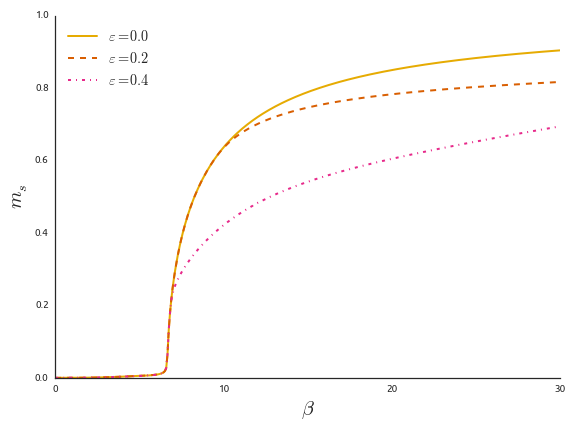
\includegraphics[scale=1.0]{phase-diagram-antiferro.png}
  \caption{Curvas da pluralidade de opiniões $m_s$ em função da pressão $\beta$ para diferentes valores da desconfiança $\ns$ e valor fixo do algorítimo de aprendizado $\rho=0.5$.
Note que conforme a desconfiança aumenta, o valor absoluto de $m_s$ cai, comportamento que se repete em $m_A$ e $m_B$, indicando a dificuldade na formação das opiniões intragrupo em situações de desconfiança.}
\end{figure}

Note que o aumento da desconfiança influencia a convicção de cada grupo em sua própria opinião, de modo que $m_s$ apresenta valores menores conforme a desconfiança $\ns$ aumenta.
Isso nos indica que a desconfiança associada às relações sociais pode ser um mecanismo que possibilita a diversidade de opiniões numa sociedade.

Para explorar essa nova possibilidade, investigaremos no capítulo \ref{ch:C3} dinâmicas para a formação de grupos dentro de uma sociedade e outros cenários em que a coexistência de grupos leva a comportamentos de interesse em eventos reais.
